\subsection{ICLab}
ICLab platform was used to conduct DNS, traceroute, TCP connect, TLS handshake and HTTP GET measurements. All except the traceroute experiments were successful.
\subsubsection{DNS} DNS queries for each domain on our list were sent from the Iranian VP to two different resolvers. A local resolver of the VP's choosing and the google resolver, 8.8.8.8 were used. A python script was then used to compare the DNS responses from a U.S. VP to the responses obtained in Iran.\\ 
In Iran, all queries using the google resolver yielded a null response. We hypothesize the DNS packets destined to 8.8.8.8 are being dropped. Some queries using the local resolver also yielded a null response even though a valid IP is obtained for the query sent by the U.S-based VP. On the flip side, a few domains in our test list got null response in the U.S. and a valid IP in Iran. Many domains that got a null response in the U.S. but not in Iran are Persian websites, though not all. To our surprise, we are able to reach some of the websites that give a null DNS response for the centinel tool when we type the domain name directly in the browser. We are uncertain what might be causing this. Figure~\ref{fig:DNSCompare} shows a comparison of DNS responses from a US VP and a Iranian VP. A large portion of the DNS queries resulted in the same response both in Iran and the U.S. As we report later, some of the websites with a valid DNS response are eventually blocked via HTTP filtering. \\
DNS queries from Iran for forty-eight different urls, most of them belonging to blogspot.com, in our test list elicited a response of 10.10.34.36, a private IP. This makes a major portion of the differenent DNS responses seen between the U.S. and Iran. We later report similar findings about private IPs when using RIPE atlas. \\

\begin{figure}
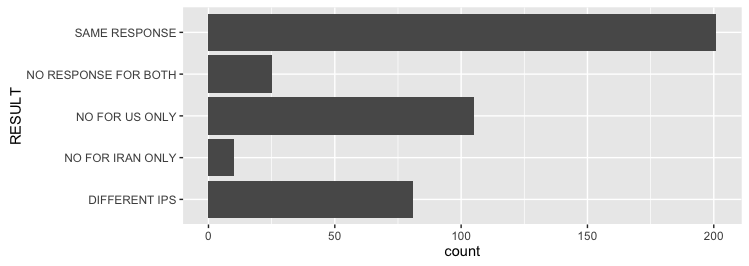
\includegraphics[
  height=.5\columnwidth,
  width=.9\columnwidth
]{pictures/DNSComparision.png}
  \caption{Comparision of DNS responses between a US-based VP and an Iranian VP}
  \label{fig:DNSCompare}
\end{figure}

\subsubsection{Traceroute} We setup our experiment to conduct traceroute measurements before we handed it over to the person responsible for ICLab. Our intention was to pinpoint the locations of the censors within Iran’s network. However, we got ``traceroute not found or not installed" error for all of our traceroute measurements. We see this as one of the limitations of the ICLab platform when compared to RIPE Atlas. Researchers do not control the remote machines located in the test countries which means they lack a clear expectations of what kinds of tests will be successful. \\
\subsubsection{TCP connect} 
TCP connection to majority of the websites in our test list succeed form our vantage points both in the U.S. and in Iran. There were only a handful of cases where TCP connection only succeed in one of the countries or failed in both. Private IPs such as 10.10.34.36 were only returned by Iranian resolvers and TCP connection to private IPs was successful in Iran. Based on our results and as previously studied by Halderman et al., we find that censorship in Iran doesn't occur at the transport layer. It occurs at the application/HTTP layer or via DNS.
\subsubsection{TLS handshake}
Both the Iranian and the U.S. VPs attempted a TLS handshake with the domains in our test list, regardless of whether the domain name started with an `https' or not. \\
Among the domains that were able to attempt the TLS handshake, there was a fifty-fifty split between the number of websites that were able to successfully complete the handshake and those that were not. It should be noted that the majority of the domains in our list come from Citizen lab test list and have a greater probability of being censored. Table~\ref{tab:error} sums up our results from the TLS handshake. Some errors such as `Connection refused' occurred exclusively in Iran whereas errors such as `TLSV1\_ALERT\_INTERNAL\_ERROR' occcured with equal frequency in both countries.\\
\begin{table}
  \caption{Errors and their number of occurrences for TLS Handshake}
  \label{tab:error}
  \begin{tabular}{ |p{5cm} |p{1cm} | p{1cm} |}
    \hline\hline
    Error Type&Iran&U.S.\\
    \hline
    {[Errno 111]} Connection refused&36&0\\
	unknown protocol (\_ssl.c:590)&19&15\\
	sslv3 alert handshake failure (\_ssl.c:590)&4&4\\
	 tlsv1 alert internal error (\_ssl.c:590)&21&21\\
	EOF occurred in violation of protocol (\_ssl.c:590)&2&2\\
	{[Errno -2]} Name or service not known&1&0\\
	{[Errno 110]} Connection timed out&93&0\\
	{[Errno 104]}Connection reset by peer&7&0\\
	{[Errno 101]}Network is unreachable&21&0\\
	{[Errno 113]} No route to host&2&0\\
 \hline
\end{tabular}
\end{table}

\subsubsection{HTTP}
 HTTP GET requests were sent from VPs in both the United States and Iran to use as control and experiment results, respectively. The same test list of more than 500 urls was used. HTTP GET requests to invalid domains were used to verify Deep Packet Inspection(DPI). To verify DPI, paths to Alexa top websites in Iran were modified with a trigger word such as `porn'. The expectation is that an invalid domain should return a 404 Page Not Found Error.\\
Based on our measurements, we find that HTTP GET requests is the most prominent mode of censorship in Iran. Many domains with successful TCP handshake gave 4xx response for a GET request. We believe that the TCP connect succeeds because the collateral damage of IP-based blocking has deterred Iran from conducting IP-based blocking. Figure~\ref{fig:TCPcomapreHTTP} shows this comparison of successful HTTP requests and successful TCP connect requests as seen from a VP in Iran. Our results show a significantly larger number of successful TCP connections compared to a successful HTTP connection. We consider an HTTP connection to be successful if the status code of the response is either 2xx or 3xx.\\
While a mix of status codes 200, 400, 3xx, 403 and 404 were obtained from the Iranian VP, the same test list of URLs resulted in a negligible number of failures when run from a U.S-based VP. A handful of error responses gotten for the US VP were usually 404 Page Not Found or 403 Forbidden. 404 error occurred mostly when the domain name was intentionally invalid like in the case of path modification to check for deep packet inspection. Some websites such as http://ladysun.net- a Women's rights website, http://www.alrased.net/site- a minority faith website, http://www.jawanan.org and http://www.jebhemelli.org- two political reform websites and a few other websites elicited a 403 response even from a VP located in the US. A traceroure measurement and geoIP lookup located the destination servers of these sites to be in countries such as Japan and the U.S. The reason for this censorship is unknown to us and would be a good thing to look at in future studies.\\
\begin{figure*}
 \centerline{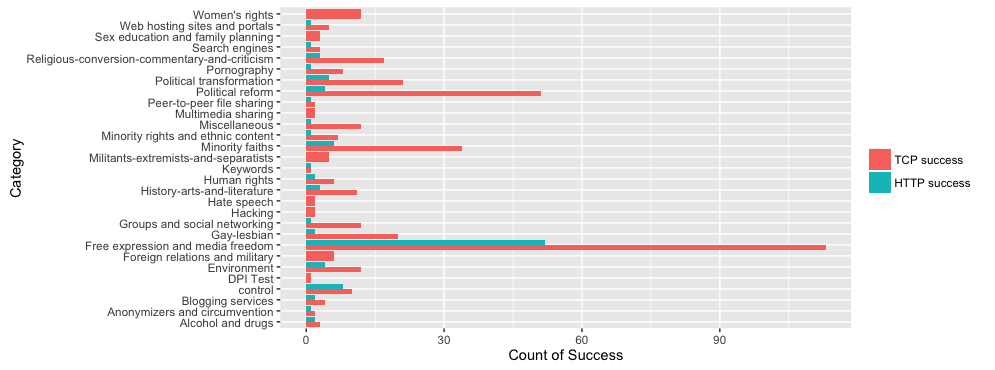
\includegraphics[width=.9\textwidth,keepaspectratio]{pictures/TCPcompareHTTP.png}}
  \caption{Comparision of successful TCP and successful HTTP requests by category}
  \label{fig:TCPcomapreHTTP}
\end{figure*}
We successfully verified the use of DPI by Iran. An invalid domain should return a 404 Page Not Found Error, however, the invalid domains which had a trigger word in the path resulted in a 403 Forbidden response. Adding `/porn' to a path always resulted in a 403 Forbidden response from Iranian VP and 404 Not Found response from a U.S-based VP. Some of our path modifications such as adding `/adult' gave a 404 response in Iran instead of the expected 403 response. This might be because `adult' is not a trigger word in Iran. Our choice of possible trigger words was obtained through online research.\\ 


